


%Table 3. Illustration of the power of the 'matrix approach to symmetry'
%The initial cell was originally tested by Himes & Mighell (1987a). BLAF confirmed the reported cubic F-centred cell with a = 15.728 A
%and, in addition, calculated the estimated error in the cell edge and produced the admitted subgroup sequence. The
%output for cells 2-5 has been shortened and rearranged. The execution time on the PDI 1/44 computer was 9.8 s.
%INITIAL UNIT CELL DATA
%. . . . . . . . . . . . . . . . . . . . . . . . . . . . . . . . . . . . . . . .
%. . . . . . . . . . . . . . . . . . . . . . . . . . . . . . . . . . . . . . . .
%Real parameters and errors
%a = 19.2600(9) alpha = 5.7696(134)
%b = 63.8825(62) beta = 19.4709(129)
%c = 27.2394(27) gamma = 17.2952(126)
%
%SEL_2025-09-18.11_13_13_2314_0.svg
%SEL_2025-09-18.11_13_13_2314_0_fit_plots.svg
%




%------------------------------------------------------------------------------
% Template file for the submission of papers to IUCr journals in LaTeX2e
% using the iucr document class
% Copyright 1999-2013 International Union of Crystallography
% Version 1.6 (28 March 2013)
%------------------------------------------------------------------------------

\documentclass[preprint]{iucr}              % DO NOT DELETE THIS LINE
%\documentclass[]{iucr}              % DO NOT DELETE THIS LINE
\usepackage{amssymb}
\usepackage{bm}
\usepackage[fleqn]{amsmath}
\DeclareGraphicsRule{.tif}{png}{.png}{`convert #1 `basename #1 .tif`.png}
%\usepackage{amsbsy}
\usepackage{float}
\usepackage{url}
%\usepackage{yfonts}
\usepackage{graphicx}
\usepackage{xcolor}
\usepackage[outdir=./]{epstopdf}
\usepackage{epsfig}
\usepackage{booktabs}
\usepackage{makecell}

\newcommand{\SVI}[0]{$\mathbf{S^{6}}$}
\newcommand{\GVI}[0]{$\bf{G^{6}}$}
\newcommand{\scalarsub}[2]{$#1_#2$}
\newcommand{\vdotv}[2]{${{\bf #1 \cdot #2}}$}
\newcommand{\charseq}[1]{({\bf #1})}

%-------------------------------------------------------------------------
% Information about journal to which submitted
%-------------------------------------------------------------------------
\journalcode{A}              % Indicate the journal to which submitted
%   A - Acta Crystallographica Section A
%   B - Acta Crystallographica Section B
%   C - Acta Crystallographica Section C
%   D - Acta Crystallographica Section D
%   E - Acta Crystallographica Section E
%   F - Acta Crystallographica Section F
%   J - Journal of Applied Crystallography
%   M - IUCrJ
%   S - Journal of Synchrotron Radiation

\begin{document}                  % DO NOT DELETE THIS LINE
	
%	Claude.ai suggestions 10125-04-13
%	I've reviewed your paper on Bravais lattice determination using the SELLA algorithm, and I have several suggestions for improvements:
%	
%	Consistency in terminology: There are variations between "Delaunay" and "Delone" throughout the paper. While you note that Delaunay later changed his name's spelling, consistency within the paper would be helpful. Perhaps use one version with a note about the alternative spelling at first mention.
%	Incomplete sections: Several sections are marked as incomplete:
%	
%	Section 3.1.1 has a note "LCA–need to normalize the vectors..."
%	Section 3.1.2 has "LCA write pseudocode for Fraction."
%	Section 6 "LCA this section is incomplete. Table needs caption/label."
%	Sections 7 and 8 are just headings without content.
%	
%	
%	Figure numbering: There appear to be duplicate Figure 1 entries - one on page 15 and another on page 16, both showing the Bravais tetrahedron.
%	Table numbering: Table 4 appears without a proper caption on page 13.
%	Equation formatting: Many mathematical expressions could benefit from proper equation formatting, particularly in the algorithm descriptions.
%	References: Some references in the text don't match entries in the reference list, and some citations don't follow a consistent format.
%	Structural organization: The paper would benefit from clearer delineation between the theoretical foundations and the practical algorithm implementation.
%	Typographical errors: Several minor typographical issues:
%	
%	"Imangine a plane" instead of "Imagine a plane" (page 12)
%	"the distance fomaverage value" instead of "from average value" (page 12)
%	"LCA," notes to self should be removed for publication
%	
%	
%	Technical clarity: The step-by-step description of the algorithm in Section 3 could be improved with clearer pseudocode or examples.
%	Figure descriptions: Figures 5-7 need more detailed captions explaining what is being visualized and how to interpret the colored points.
%	
%	I hope these suggestions are helpful for improving your manuscript.
	
	
	%-------------------------------------------------------------------------
	% The introductory (header) part of the paper
	%-------------------------------------------------------------------------
	
	% The title of the paper. Use \shorttitle to indicate an abbreviated title
	% for use in running heads (you will need to uncomment it).
	
	{\LARGE \emph{\today}} \\
	
\cauthor[a]{Lawrence C.}{Andrews}{larry6640995@gmail.com}{}
\author[a]{Herbert J.}{Bernstein}
\author[b]{Nicholas K.}{Sauter}

\aff[a]{Ronin Institute for Independent Scholarship 2.0, USA}
\aff[b]{Lawrence Berkeley National Laboratory, 1 Cyclotron Rd., Berkeley 94720, CA, USA}

\shortauthor{Andrews, Bernstein, and Sauter}

\title{Determining Bravais Lattice Types Using Selling Reduction}

\maketitle
	
	%\shorttitle{SELLA  Determining Bravais Lattice Types}
	
	% Authors' names and addresses. Use \cauthor for the main (contact) author.
	% Use \author for all other authors. Use \aff for authors' affiliations.
	% Use lower-case letters in square brackets to link authors to their
	% affiliations; if there is only one affiliation address, remove the [a].
	
	
	% ORCID for LCA - 0000-0002-4451-1641
	
\aff[a]{Ronin Institute for Independent Scholarship 2.0, USA}
\aff[b]{Lawrence Berkeley National Laboratory, 1 Cyclotron Rd., Berkeley 94720, CA, USA}


	% Use \shortauthor to indicate an abbreviated author list for use in
	% running heads (you will need to uncomment it).
	
	\shortauthor{Andrews, Bernstein, and Sauter}
	
	% Use \vita if required to give biographical details (for authors of
	% invited review papers only). Uncomment it.
	
	% lca IUCr id IUCr6401
	%\vita{Author's biography}
	
	% Keywords (required for Journal of Synchrotron Radiation only)
	% Use the \keyword macro for each word or phrase, e.g. 
	% \keyword{X-ray diffraction}\keyword{muscle}
	
	%\keyword{keyword}
	\keyword{Unit cell reduction}
	\keyword{Delaunay}
	\keyword{Delone}
	\keyword{Niggli}
	\keyword{Selling}
	\keyword{Bravais Lattice}
	
	% PDB and NDB reference codes for structures referenced in the article and
	% deposited with the Protein Data Bank and Nucleic Acids Database (Acta
	% Crystallographica Section D). Repeat for each separate structure e.g
	% \PDBref[dethiobiotin synthetase]{1byi} \NDBref[d(G$_4$CGC$_4$)]{ad0002}
	
	%\PDBref[optional name]{refcode}
	%\NDBref[optional name]{refcode}	



\begin{abstract}
	SELLA is a straightforward algorithm for determining Bravais lattice type
	based on Selling (Delone) reduction. The method represents each Bravais type
	as one or more linear manifolds in the six-dimensional space $S^6$ of Selling
	scalars. Distances from a probe cell to these manifolds are computed using
	projectors and their orthogonal complements, giving a clear metric of fit.
	The geometry of $S^6$ provides a simple, convex reduced domain, making it
	well suited for treating experimental error and approximate symmetry. The
	24 Delone types described by Delaunay (1932) appear naturally in this
	framework. Examples and tests against large data sets are included.
\end{abstract}

\section{Introduction}

Determining the Bravais lattice type from measured unit-cell parameters is a
routine crystallographic task, but the presence of experimental error and
near-symmetry can complicate the process. The traditional approach uses the
metric tensor in $G^6$ together with Niggli reduction (Niggli, 1928). While
mathematically correct, the geometry of the Niggli-reduced region is
complicated: it is non-convex, some facets are open while others are closed,
and higher-order intersections require special handling. These features make
it difficult to treat perturbations in a uniform way.

Selling (Delone) reduction provides a simpler geometric setting. The six
Selling scalars form a point in the linear space $S^6$, and the Selling-reduced
domain is the all-negative orthant of that space. The domain is convex, the
boundary operations are uniform, and reflections act linearly. These
properties make $S^6$ a natural place to study approximate symmetry and to
measure distances between lattices.

In this paper we describe SELLA, an algorithm for Bravais lattice
determination based on Selling reduction. Each Bravais type is represented by
one or more linear manifolds in $S^6$, and the distance from a probe cell to
any type is obtained from the orthogonal complement of the corresponding
projector. The method behaves smoothly under perturbations of the input cell
and provides a clear metric of fit.

The 24 Delone types described by Delaunay (1932) appear naturally in this
framework. We describe their representation in $S^6$, the construction of the
associated projectors, and the use of these projectors to classify experimental
cells. Examples and tests against large data sets are included.

\section{Geometry of Reduction: Niggli vs.\ Selling}

\subsection{Niggli reduction and the geometry of $G^6$}

Niggli reduction provides a unique reduced cell for triclinic lattices by
imposing a hierarchy of inequalities and equalities on the metric tensor.
These rules define a canonical region of $G^6$, but the geometry of this
region is intricate. It is non-convex, and its boundaries mix open and closed
facets. Ambiguities arise when several boundary conditions are simultaneously
active, because the original tie-breaking rules were written for
single-condition boundaries. As a result, the mapping from an experimental
cell to its reduced form can become non-unique near higher-order
intersections.

These complications have practical consequences. Grosse-Kunstleve, Sauter,
and Adams (2004) documented stability problems and infinite-loop behavior
near certain boundaries. Although the boundary structure is well defined—the
standard table lists 45 polytopes in $G^6$—the reduction rules do not always
specify how to choose among equivalent representatives on their
intersections.

\subsection{Selling reduction and the geometry of $S^6$}

Selling (Delone) reduction embeds the six Selling scalars as coordinates in
the linear space $S^6$. The Selling-reduced domain is simply the convex,
closed, all-negative orthant of that space. Boundary operations are uniform,
and reflections act linearly. As in $G^6$, each Bravais type corresponds to a
finite collection of linear manifolds, each determined by a particular pattern
of equalities or zeros in the scalars. The advantage of $S^6$ lies in the
geometry of the reduced domain: the manifolds can be enumerated
systematically without the complications introduced by the Niggli region.

\subsection{Definitions of $G^6$ and $S^6$}

The space $G^6$ is the six-dimensional real vector space of metric tensors for
unit cells, expressed in terms of scalar products of the edge vectors
$\mathbf{a}, \mathbf{b}, \mathbf{c}$. A point $\mathbf{g} \in G^6$ is defined by


\[
\mathbf{g} = (g_1, g_2, g_3, g_4, g_5, g_6)
= \left( \mathbf{a}\!\cdot\!\mathbf{a},\,
\mathbf{b}\!\cdot\!\mathbf{b},\,
\mathbf{c}\!\cdot\!\mathbf{c},\,
2\,\mathbf{b}\!\cdot\!\mathbf{c},\,
2\,\mathbf{a}\!\cdot\!\mathbf{c},\,
2\,\mathbf{a}\!\cdot\!\mathbf{b} \right).
\]


The first three components represent squared edge lengths; the last three
encode interaxial angles via scalar products scaled by a factor of~2.

The space $S^6$ is the six-dimensional real vector space of Selling scalars
derived from scalar products among the four vectors
$\mathbf{a}, \mathbf{b}, \mathbf{c}, \mathbf{d}$, where
$\mathbf{d} = -\mathbf{a} - \mathbf{b} - \mathbf{c}$. A point
$\mathbf{s} \in S^6$ is defined by


\[
\mathbf{s} = (s_1, s_2, s_3, s_4, s_5, s_6)
= \left( \mathbf{b}\!\cdot\!\mathbf{c},\,
\mathbf{a}\!\cdot\!\mathbf{c},\,
\mathbf{a}\!\cdot\!\mathbf{b},\,
\mathbf{a}\!\cdot\!\mathbf{d},\,
\mathbf{b}\!\cdot\!\mathbf{d},\,
\mathbf{c}\!\cdot\!\mathbf{d} \right).
\]


Selling reduction places all reduced cells in the all-negative orthant of
$S^6$, giving a convex domain with uniform boundary behavior.

\section{Overview of SELLA}

SELLA is based on the observation that each Bravais type corresponds to one
or more linear manifolds in $S^6$. For each manifold, a projector is
constructed that maps any vector in $S^6$ to the closest point on that
manifold in the least-squares sense. The orthogonal complement of the
projector (the ``perp'') measures the distance from a probe cell to the
manifold.

The algorithm proceeds by generating all representations of all non-triclinic
Delone types within the Selling-reduced domain, including those obtained by
boundary transforms. For each representation, a projector is computed. Given a
probe cell, its Selling-reduced vector is compared to each manifold by
applying the corresponding perp. The Bravais type(s) with the smallest
distance are reported.

The method is complete in the sense that all relevant manifolds are included,
and continuous in the sense that small perturbations of the input cell lead to
small changes in the computed distances.


\section{Historical Background}

Bravais (1850) classified lattices into 14 types based on geometric symmetry.
Delaunay (1932) refined this classification by examining the Dirichlet (Voronoi)
cell of the lattice and introduced 24 types, now called the Delone types. Several
of these correspond to the same Bravais type, but the Delone classification is
useful because it describes the local geometry of the lattice in a uniform way.

Selling (1874) introduced a reduction method based on six scalar products among
the vectors $\mathbf{a}, \mathbf{b}, \mathbf{c}, \mathbf{d}$, where
$\mathbf{d} = -\mathbf{a} - \mathbf{b} - \mathbf{c}$. Delaunay adopted these
scalars in his formulation of reduction. Andrews et al.\ (2019a, 2019b) later
showed that the Selling scalars form a natural coordinate system for a metric
space $S^6$ in which distances between lattices can be measured directly.

Zimmermann and Burzlaff (1985) used Selling scalars in their program DELOS,
treating the scalars as a list of six numbers. SELLA extends this idea by treating
the scalars as points in a linear space, allowing the use of projectors and
orthogonal complements to measure distances to the Bravais manifolds.

The 24 Delone types appear naturally in $S^6$, and their representation as linear
manifolds provides a convenient framework for classification. Three of the Delone
types (M3, M2B, and O3) correspond to boundaries between other types and do not
represent unique Bravais types.

\section{Terminology and Representations}

\subsection{The Bravais tetrahedron}

Delaunay represented the Selling scalars using a tetrahedron whose edges are
labeled by the six scalar products. This diagram, often called the Bravais
tetrahedron, provides a compact way to visualize which scalars are zero or which
pairs are equal. The labeling conventions have varied in the literature; Table~1
summarizes several of these.

\subsection{Characters}

For reduced cells in $S^6$, each Bravais type is represented by a linear manifold
that includes the origin. The structure of the manifold is described by its
\emph{character}, a symbolic representation indicating which scalars are zero and
which are equal. For example, the character for the rhombohedral type H1 is
\((rrr\,sss)\), indicating two triplets of equal values. The primitive monoclinic
type M4 has character \((00r\,stu)\), indicating two zeros and four independent
values.

Characters provide a compact way to describe the geometry of each manifold and
are useful for generating sample vectors and constructing projectors.

\subsection{Zero patterns and equal-value multiplets}

A zero in a Selling scalar indicates that the corresponding vector lies on a
boundary of the Selling-reduced orthant. Equal-value multiplets indicate
additional symmetry. For example, the orthorhombic type O5 has character
\((000\,rst)\), with three zeros and three independent values.

These patterns determine the dimension of the manifold and the structure of the
projector associated with the type.

\subsection{Delone types and Bravais types}

The 24 Delone types refine the 14 Bravais types. Some Bravais types correspond to
multiple Delone types; for example, the cubic Bravais type includes three Delone
types (C1, C3, C5). Three Delone types (M3, M2B, O3) correspond to boundaries
between other types and do not represent unique Bravais types.

SELLA uses the Delone types as the fundamental units for classification, since
each Delone type corresponds to a single linear manifold in $S^6$.

\section{Geometry of Bravais Manifolds in \SVI{}}

Each Bravais type corresponds to one or more linear manifolds in $S^6$. These
manifolds are defined by the zero patterns and equal-value multiplets in the
character. For example, the manifold for M4 consists of all vectors of the form
\((0,0,r,s,t,u)\) with $r,s,t,u < 0$.

The manifolds are linear because the Selling scalars are linear functions of the
metric tensor. The Selling-reduced domain is the all-negative orthant, so each
manifold is the intersection of a linear subspace with this orthant.

\subsection{Dimension}

The dimension of a manifold is determined by the number of independent scalars.
For example:
\begin{itemize}
	\item M4 has two zeros and four independent values, so its manifold is
	four-dimensional.
	\item O5 has three zeros and three independent values, so its manifold is
	three-dimensional.
	\item H1 has two triplets of equal values, so its manifold is two-dimensional.
\end{itemize}

\subsection{Degenerate types}

Three Delone types (M3, M2B, O3) correspond to boundaries between other types.
These manifolds have reduced dimension and do not represent unique Bravais
types. A probe cell close to one of these manifolds will also be close to one or
both of the adjacent manifolds.

\subsection{Reflections and boundary transforms}

The 24 reflections of $S^6$ correspond to permutations and sign changes of the
Selling scalars. These reflections map each manifold to 24 equivalent copies.
Boundary transforms occur when a scalar crosses zero; these transforms map a
vector on one side of a boundary to a vector on the other side. The transforms
are linear and self-inverse.

\subsection{Continuity}

Because the manifolds are linear and the domain is convex, distances from a
probe cell to the manifolds vary continuously with the input cell. This is
important for treating experimental error and approximate symmetry. For
example, varying the two zero scalars in M4 over a circle in the $(s_1,s_2)$
plane produces a continuous curve of distances to the M4 manifold.

Similarly, varying the three zeros in O5 over a sphere produces a continuous
surface of distances. These continuity properties are used in Section~8 to
demonstrate the completeness of SELLA.


\section{The SELLA Algorithm}

SELLA classifies a probe cell by measuring its distance to the manifolds
associated with the Delone types. The algorithm has three main components:
generation of sample vectors, construction of projectors and perps, and
evaluation of distances.

\subsection{Generating sample vectors}

Each Delone type is represented by a linear manifold in $S^6$. To construct a
projector for a type, we begin by generating a representative vector for that
manifold.

\paragraph{Step 1: Initial vector.}
Choose a random vector in $S^6$ with no zeros and no duplicate values. The
values should be large enough that adding or subtracting the smallest
representable floating-point number (DBL\_MIN) does not change them. This
value will later be used to mark positions of zeros.

\paragraph{Step 2: Apply projectors.}
For each Delone type, multiply the initial vector by the projector associated
with that type. The result is a sample vector lying on the manifold.

\paragraph{Step 3: Boundary transforms and reflections.}
If the sample vector contains zeros, apply the appropriate boundary transform
for each zero. Because boundary transforms do not commute, all orderings must
be considered. For each transformed vector, generate the 24 reflections
(permutations and sign changes allowed by Selling reduction). Store all
results.

This process generates a complete set of sample vectors for each Delone type.
Duplicates are removed at the end.

\subsection{Constructing projectors and perps}

Each sample vector encodes the structure of its manifold through its zeros and
duplicate values. A projector matrix is constructed as follows.

\paragraph{Step 1: Zero DBL\_MIN entries.}
Any entry equal to DBL\_MIN is set to zero.

\paragraph{Step 2: Diagonal entries.}
For each scalar $s_i$,


\[
m_{ii} =
\begin{cases}
	0, & \text{if } s_i = 0 \text{ or } \mathrm{Fraction}(s_i) = 0, \\
	\mathrm{Fraction}(s_i), & \text{otherwise},
\end{cases}
\]


where $\mathrm{Fraction}(s_i)$ is the reciprocal of the number of occurrences
of the value $s_i$ in the vector.

\paragraph{Step 3: Off-diagonal entries.}
For $i \neq j$,


\[
m_{ij} =
\begin{cases}
	\mathrm{Fraction}(s_j), & \text{if } s_i = s_j \text{ or } |s_j| > 0, \\
	0, & \text{otherwise}.
\end{cases}
\]



The perp for the manifold is obtained by subtracting the projector from the
identity matrix. The norm of the perp applied to a probe vector gives the
distance from the probe to the manifold.

\subsection{Evaluating a probe cell}

Given a probe cell:

\begin{enumerate}
	\item Convert the cell to its Selling-reduced form in $S^6$.
	\item Apply each perp to the probe vector.
	\item Compute the norm of each result.
	\item Identify the Delone type(s) with the smallest distance.
\end{enumerate}

The corresponding Bravais type is reported. If the probe lies near a degenerate
Delone type, two adjacent types may be returned.

\section{Completeness and Correctness}

SELLA is complete in the sense that every relevant manifold is included in the
library of projectors. The justification has three parts.

\subsection{Coverage of the fundamental unit}

All Bravais lattice types within the Selling-reduced domain (all scalars
negative) have their projectors generated. The 24 reflections of a reduced cell
cover all equivalent representations. Points near boundaries are handled by
boundary transforms.

\subsection{Boundary transforms preserve proximity}

Consider a probe cell infinitesimally close to a manifold with one zero scalar.
Let $p$ be the closest point on the manifold. Applying the boundary transform
to both $p$ and the probe produces a new pair of points in a different
representation of the same type. The distance between them remains
infinitesimal. This argument extends to cases with two or three zeros.

\subsection{No missing manifolds}

Suppose a probe lies outside the fundamental unit but is near an undiscovered
manifold. If the probe is near a boundary defined by a single zero, applying
the boundary transform moves both the probe and the manifold into the
fundamental unit. Since all manifolds within and on the boundaries of the
fundamental unit have been generated, the putative manifold must already be in
the library. The same reasoning applies to cases with two or three zeros.

Thus, after applying all boundary transforms and reflections, no manifold is
missed. In total, 239 non-triclinic manifolds are generated (249 if triclinic
cases are included).

\section{Validation Against Data}

To test SELLA, 89\,539 unit cells were extracted from the Protein Data Bank
(Bernstein et al., 1977; Berman et al., 2000). Each cell was Selling-reduced
and classified using SELLA.

All but 57 cells were found at zero distance from their assigned Bravais type.
The 57 exceptions were identified as incorrect unit cells for their assigned
types. The distances were small, indicating modest deviations from the correct
parameters. These cases were later corrected (Burley, 2018).

Table~3 lists the 57 cells, their assigned types, and their distances.

\section{Comparisons}

Several measures have been proposed for comparing unit cells. Table~4 compares
SELLA distances with:

\begin{itemize}
	\item the $G^6$ distance,
	\item the BGAOL $Z$ score,
	\item the XDS quality index (QI),
	\item a scaled version of QI.
\end{itemize}

SELLA provides a direct geometric measure in $S^6$ and behaves smoothly under
perturbations. The examples in Table~4 illustrate that SELLA distances correlate
well with other measures while providing a clear interpretation as the distance
to a linear manifold.


\section{Discussion}

SELLA provides a uniform geometric framework for Bravais lattice
determination. The use of $S^6$ avoids the complications of the Niggli-reduced
region in $G^6$, where non-convexity and mixed open/closed boundaries require
special handling. In contrast, the Selling-reduced domain is convex, and all
boundary operations are linear and self-inverse. This makes it straightforward
to enumerate all representations of each Delone type and to construct the
corresponding projectors.

The projector–perp formulation gives a clear metric of fit. The distance from a
probe cell to a Bravais type is simply the norm of the perp applied to the
Selling-reduced vector. This distance behaves smoothly under perturbations,
making the method suitable for experimental data. The examples in Section~9
show that SELLA identifies incorrect unit cells reliably and that the distances
provide a meaningful measure of deviation.

The method is also computationally efficient. Once the library of projectors is
constructed, classification of a probe cell requires only matrix–vector
multiplications. The number of projectors is modest (239 non-triclinic types),
and the operations are inexpensive.

\section{Conclusion}

SELLA uses Selling reduction and the geometry of $S^6$ to provide a simple and
complete method for Bravais lattice determination. Each Bravais type is
represented by one or more linear manifolds, and distances to these manifolds
are computed using projectors and their orthogonal complements. The method
handles experimental error and approximate symmetry in a uniform way and
produces clear, interpretable metrics of fit.

The 24 Delone types appear naturally in this framework, and the method
correctly identifies all types in large data sets. SELLA provides a practical
tool for crystallographers and a geometric foundation for further work on
lattice classification and comparison.

\section*{Figures}

\begin{figure}[h]
	\centering
	% \includegraphics{figure1_placeholder}
	\caption{Placeholder for Figure~1. Suggested content: Bravais tetrahedron with
		labels for the six Selling scalars.}
\end{figure}

\begin{figure}[h]
	\centering
	% \includegraphics{figure2_placeholder}
	\caption{Placeholder for Figure~2. Suggested content: schematic comparison of
		the Niggli-reduced region in $G^6$ and the Selling-reduced orthant in $S^6$.}
\end{figure}

\begin{figure}[h]
	\centering
	% \includegraphics{figure3_placeholder}
	\caption{Placeholder for Figure~3. Suggested content: example of a Bravais
		manifold in $S^6$ showing zero patterns and equal-value multiplets.}
\end{figure}

\begin{figure}[h]
	\centering
	% \includegraphics{figure4_placeholder}
	\caption{Placeholder for Figure~4. Suggested content: continuity test for a
		manifold such as M4, showing distances along a circle in the $(s_1,s_2)$ plane.}
\end{figure}

\begin{figure}[h]
	\centering
	% \includegraphics{figure5_placeholder}
	\caption{Placeholder for Figure~5. Suggested content: comparison of SELLA
		distances with other measures (G6 distance, BGAOL $Z$ score, XDS QI).}
\end{figure}
	
	
	
	
	% Appendices appear after the main body of the text. They are prefixed by
	% a single \appendix declaration, and are then structured just like the
	% body text.
	
	%-------------------------------------------------------------------------
	% The back matter of the paper - acknowledgements and references
	%-------------------------------------------------------------------------
	
	% Acknowledgements come after the appendices
	
	
	\ack{{\bf Acknowledgements}}
	Careful copy-editing and corrections by Frances C. Bernstein are 
	gratefully acknowledged.  	Our thanks to Jean Jakoncic and Alexei Soares for 
	helpful conversations and access to data and facilties at 
	Brookhaven National Laboratory.
	% References are at the end of the document, between \begin{references}
		% and \end{references} tags. Each reference is in a \reference entry.
	
	\ack{{\bf Funding information}}      
	
	Funding for this research was provided in part by: US Department of Energy Offices of Biological and Environmental Research and of Basic Energy Sciences (grant No. DE-AC02-98CH10886 ; grant No. E-SC0012704); U.S. National Institutes of Health (grant No. P41RR012408; grant No. P41GM103473; grant No. P41GM111244; grant No. R01GM117126, grant No. 1R21GM129570; grant No. P30GM133893); Dectris, Ltd.
	
	\bibliographystyle{iucr}
	\bibliography{Reduced}
	
	%-------------------------------------------------------------------------
	% TABLES AND FIGURES SHOULD BE INSERTED AFTER THE MAIN BODY OF THE TEXT
	%-------------------------------------------------------------------------
	
	% Simple tables should use the tabular environment according to this
	% model
	
	\begin{table}
		\caption{The 21 non-triclinic Delone types with the count of permutations.
			The asterisks indicate non-crystallographic types.}
		\label{table:TypeCounts}
		\begin{tabular}{lr}
			Delone type & Count    \\
			\midrule
			H4&12\\
			C1&1\\
			C3&3\\
			C5&16\\
			H1&4\\
			H3&12\\
			T1&3\\
			T2&6\\
			T5&48\\
			O1A&3\\
			O1B&1\\
			O2&6\\
			O3*&9\\
			O4&36\\
			O5&16\\
			M1A&6\\
			M1B&3\\
			M2A&12\\
			M2B*&12\\
			M3*&18\\
			M4&12\\
			\bottomrule
		\end{tabular}
	\end{table}
	
\fontseries{Courier}{
	\begin{table}
		\caption{Properly normalized projectors for the 24 Delone types}
		\label{table:DeloneTypes}
		\begin{tabular}{lclc}
			\toprule
			Type & Lattice & Projector & Characteristic \\
			\midrule
			C1  & (cI) & [1/6 1/6 1/6 1/6 1/6 1/6/ 1/6 1/6 1/6 1/6 1/6 1/6/ 1/6 1/6 1/6 1/6 1/6 1/6/ 1/6 1/6 1/6 1/6 1/6 1/6/ 1/6 1/6 1/6 1/6 1/6 1/6/ 1/6 1/6 1/6 1/6 1/6 1/6] & (rrr rrr) \\ 
			C3  & (cF) & [1/4 1/4 0 1/4 1/4 0/ 1/4 1/4 0 1/4 1/4 0/ 0 0 0 0 0 0/ 1/4 1/4 0 1/4 1/4 0/ 1/4 1/4 0 1/4 1/4 0/ 0 0 0 0 0 0] & (rr0 rr0) \\ 
			C5  & (cP) & [0 0 0 0 0 0/ 0 0 0 0 0 0/ 0 0 0 0 0 0/ 0 0 0 1/3 1/3 1/3/ 0 0 0 1/3 1/3 1/3/ 0 0 0 1/3 1/3 1/3] & (000 rrr) \\ \\
			
			T1  & (tI) & [1/4 1/4 0 1/4 1/4 0/ 1/4 1/4 0 1/4 1/4 0/ 0 0 1/2 0 0 1/2/ 1/4 1/4 0 1/4 1/4 0/ 1/4 1/4 0 1/4 1/4 0/ 0 0 1/2 0 0 1/2] & (rrr rrs) \\ 
			T2  & (tI) & [1/4 1/4 0 1/4 1/4 0/ 1/4 1/4 0 1/4 1/4 0/ 0 0 0 0 0 0/ 1/4 1/4 0 1/4 1/4 0/ 1/4 1/4 0 1/4 1/4 0/ 0 0 0 0 0 1] & (rr0 rrs) \\ 
			T5  & (tP) & [0 0 0 0 0 0/ 0 0 0 0 0 0/ 0 0 0 0 0 0/ 0 0 0 1/2 1/2 0/ 0 0 0 1/2 1/2 0/ 0 0 0 0 0 1] & (000 rrs) \\ \\
			
			H1  & (hR) & [1/3 1/3 1/3 0 0 0/ 1/3 1/3 1/3 0 0 0/ 1/3 1/3 1/3 0 0 0/ 0 0 0 1/3 1/3 1/3/ 0 0 0 1/3 1/3 1/3/ 0 0 0 1/3 1/3 1/3] & (rrr sss) \\ 
			H3  & (hR) & [1/4 1/4 0 0 1/4 0/ 1/4 1/4 0 0 1/4 0/ 0 0 0 0 0 0/ 0 0 0 1 0 0/ 1/4 1/4 0 0 1/4 0/ 0 0 0 0 0 0] & (rr0 sr0) \\
			H4  & (hP) & [0 0 0 0 0 0/ 0 0 0 0 0 0/ 0 0 1/3 1/3 1/3 0/ 0 0 1/3 1/3 1/3 0/ 0 0 1/3 1/3 1/3 0/ 0 0 0 0 0 1] & (00r rrs) \\ \\
			
			O1A & (oF) & [1/4 1/4 0 1/4 1/4 0/ 1/4 1/4 0 1/4 1/4 0/ 0 0 1 0 0 0/ 1/4 1/4 0 1/4 1/4 0/ 1/4 1/4 0 1/4 1/4 0/ 0 0 0 0 0 1] & (rrs rrt) \\ 
			O1B & (oI) & [1/2 0 0 1/2 0 0/ 0 1/2 0 0 1/2 0/ 0 0 1/2 0 0 1/2/ 1/2 0 0 1/2 0 0/ 0 1/2 0 0 1/2 0/ 0 0 1/2 0 0 1/2] & (rst rst) \\ 
			O2  & (oI) & [1/2 0 0 0 1/2 0/ 0 1/2 0 1/2 0 0/ 0 0 0 0 0 0/ 0 1/2 0 1/2 0 0/ 1/2 0 0 0 1/2 0/ 0 0 0 0 0 1] & (rs0 srt) \\ 
			O3  & (oI) & [1/2 0 0 1/2 0 0/ 0 1/2 0 0 1/2 0/ 0 0 0 0 0 0/ 1/2 0 0 1/2 0 0/ 0 1/2 0 0 1/2 0/ 0 0 0 0 0 0] & (rs0 rs0) \\ 
			O4  & (oS) & [0 0 0 0 0 0/ 0 0 0 0 0 0/ 0 0 1 0 0 0/ 0 0 0 1/2 1/2 0/ 0 0 0 1/2 1/2 0/ 0 0 0 0 0 1] & (00r sst) \\ 
			O5  & (oP) & [0 0 0 0 0 0/ 0 0 0 0 0 0/ 0 0 0 0 0 0/ 0 0 0 1 0 0/ 0 0 0 0 1 0/ 0 0 0 0 0 1] & (000 rst) \\ \\
			
			M1A & (mC) & [1/2 1/2 0 0 0 0/ 1/2 1/2 0 0 0 0/ 0 0 1 0 0 0/ 0 0 0 1/2 1/2 0/ 0 0 0 1/2 1/2 0/ 0 0 0 0 0 1] & (rrs ttu) \\ 
			M1B & (mC) & [1/2 0 0 1/2 0 0/ 0 1/2 0 0 1/2 0/ 0 0 1 0 0 0/ 1/2 0 0 1/2 0 0/ 0 1/2 0 0 1/2 0/ 0 0 0 0 0 1] & (rst rsu) \\ 
			M2A & (mC) & [1 0 0 0 0 0/ 0 1/2 0 1/2 0 0/ 0 0 0 0 0 0/ 0 1/2 0 1/2 0 0/ 0 0 0 0 1 0/ 0 0 0 0 0 1] & (rs0 stu) \\ 
			M2B & (mC) & [1/2 0 0 1/2 0 0/ 0 1/2 0 0 1/2 0/ 0 0 0 0 0 0/ 1/2 0 0 1/2 0 0/ 0 1/2 0 0 1/2 0/ 0 0 0 0 0 1] & (rs0 rst) \\ 
			M3  & (mC) & [1 0 0 0 0 0/ 0 1/2 0 0 1/2 0/ 0 0 0 0 0 0/ 0 0 0 1 0 0/ 0 1/2 0 0 1/2 0/ 0 0 0 0 0 0] & (rs0 ts0) \\ 
			M4  & (mP) & [0 0 0 0 0 0/ 0 0 0 0 0 0/ 0 0 1 0 0 0/ 0 0 0 1 0 0/ 0 0 0 0 1 0/ 0 0 0 0 0 1] & (00r stu) \\ \\
			
			A1  & (aP) & [1 0 0 0 0 0/ 0 1 0 0 0 0/ 0 0 1 0 0 0/ 0 0 0 1 0 0/ 0 0 0 0 1 0/ 0 0 0 0 0 1] & (rst uvw) \\ 
			A2  & (aP) & [1 0 0 0 0 0/ 0 1 0 0 0 0/ 0 0 0 0 0 0/ 0 0 0 1 0 0/ 0 0 0 0 1 0/ 0 0 0 0 0 1] & (rs0 tuv) \\ 
			A3  & (aP) & [1 0 0 0 0 0/ 0 1 0 0 0 0/ 0 0 0 0 0 0/ 0 0 0 1 0 0/ 0 0 0 0 1 0/ 0 0 0 0 0 0] & (rs0 tu0) \\ \\				
			\bottomrule
		\end{tabular}
	\end{table}
}
	% Postscript figures can be included with multiple figure blocks
	
	
	\begin{figure}
		\caption{Bravais tetrahedron with labeling as used in the International Tables}
		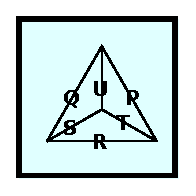
\includegraphics[width=3cm]{PQRSTU}
		\label{fig:PQRSTU}
	\end{figure}
	
		
	%	\begin{figure}
		%		\caption{The Delone types}
		%		\label{fig:DeloneTypes}
		%		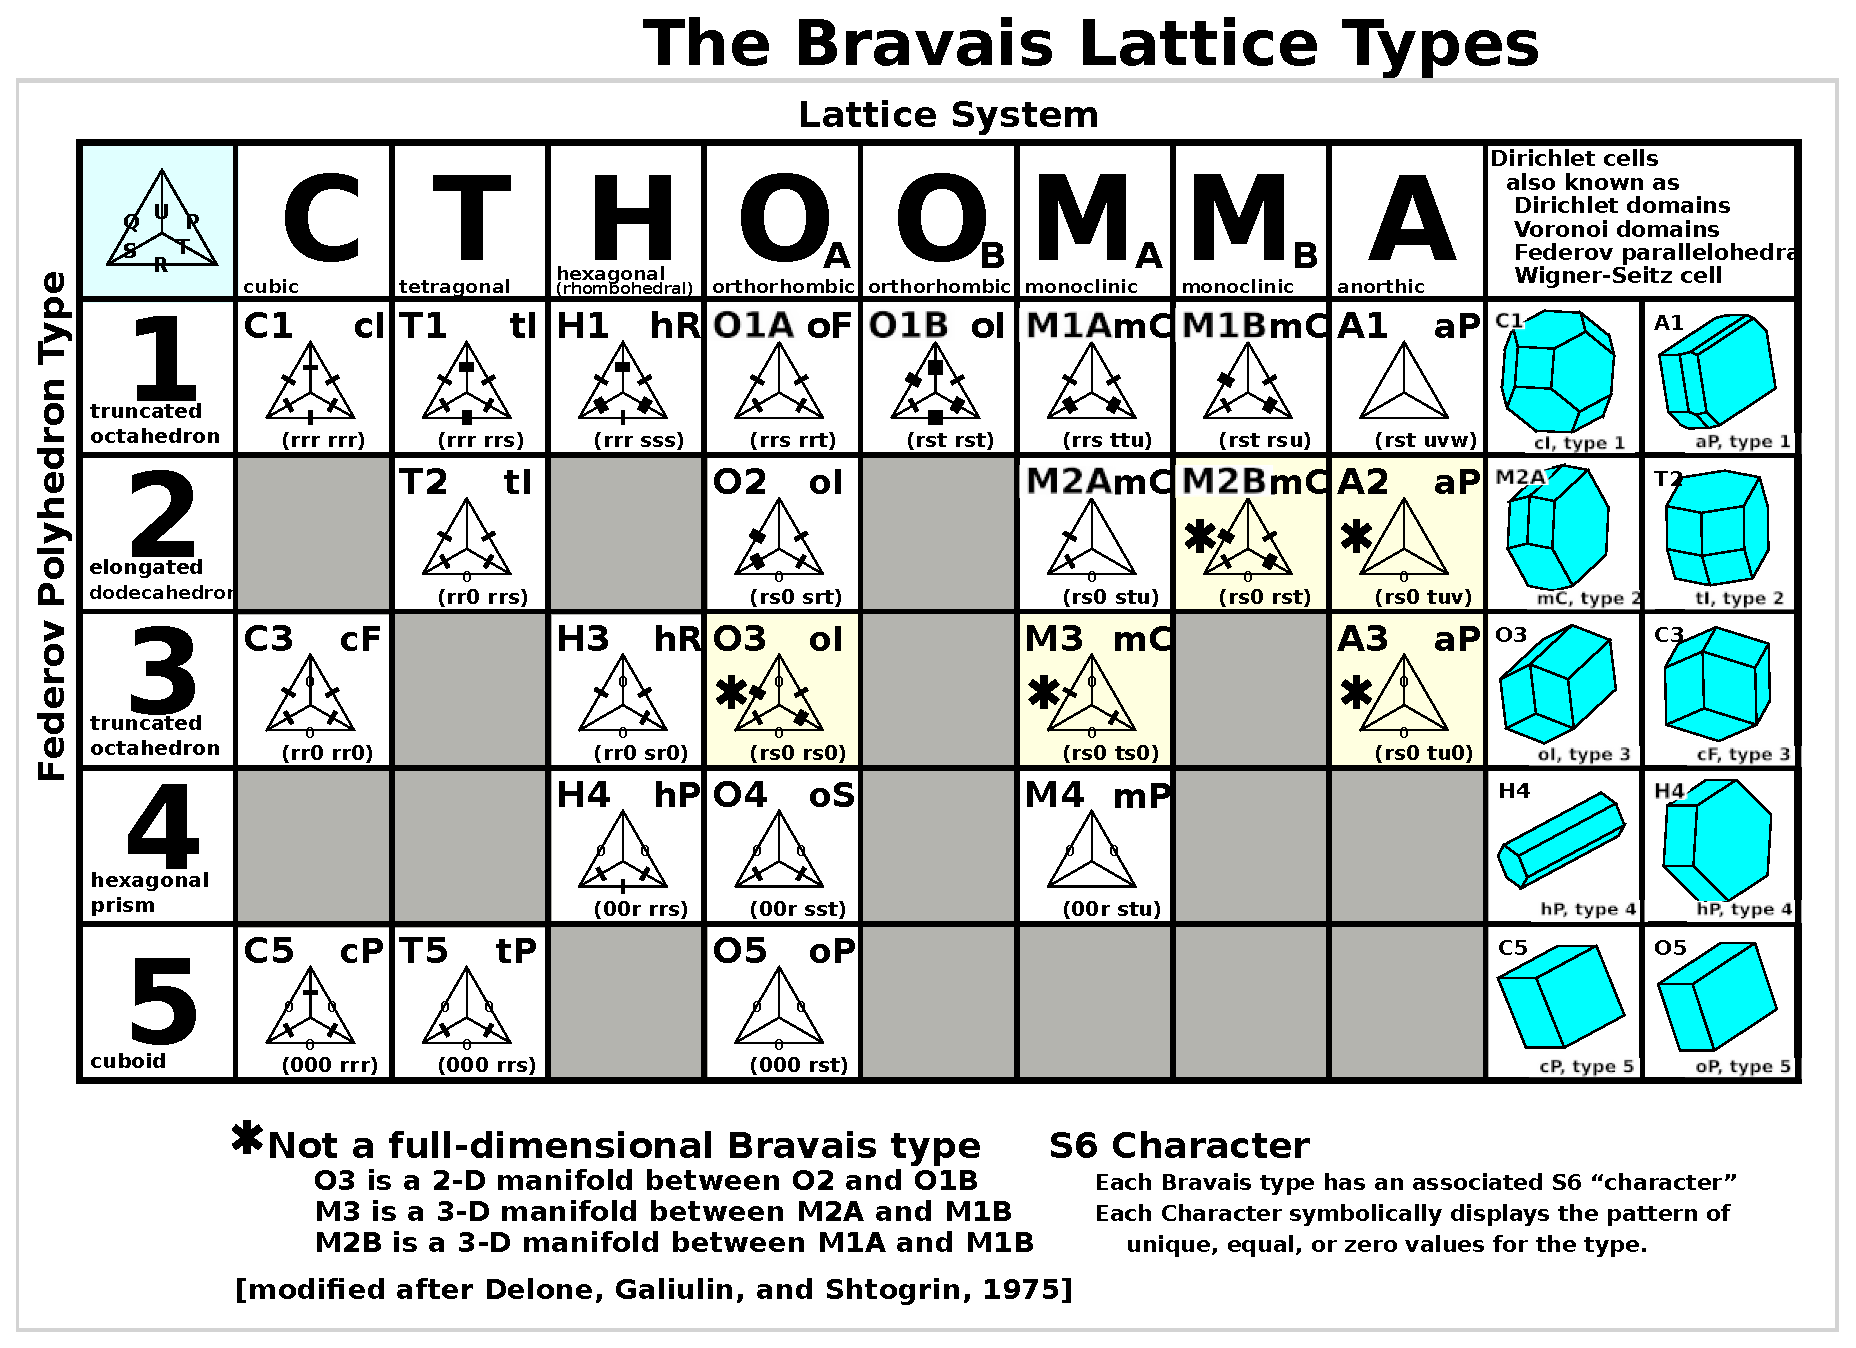
\includegraphics[width=12cm]{DeloneGridClaude_2-3}
		%	\end{figure}
	\begin{figure}
		\centering
		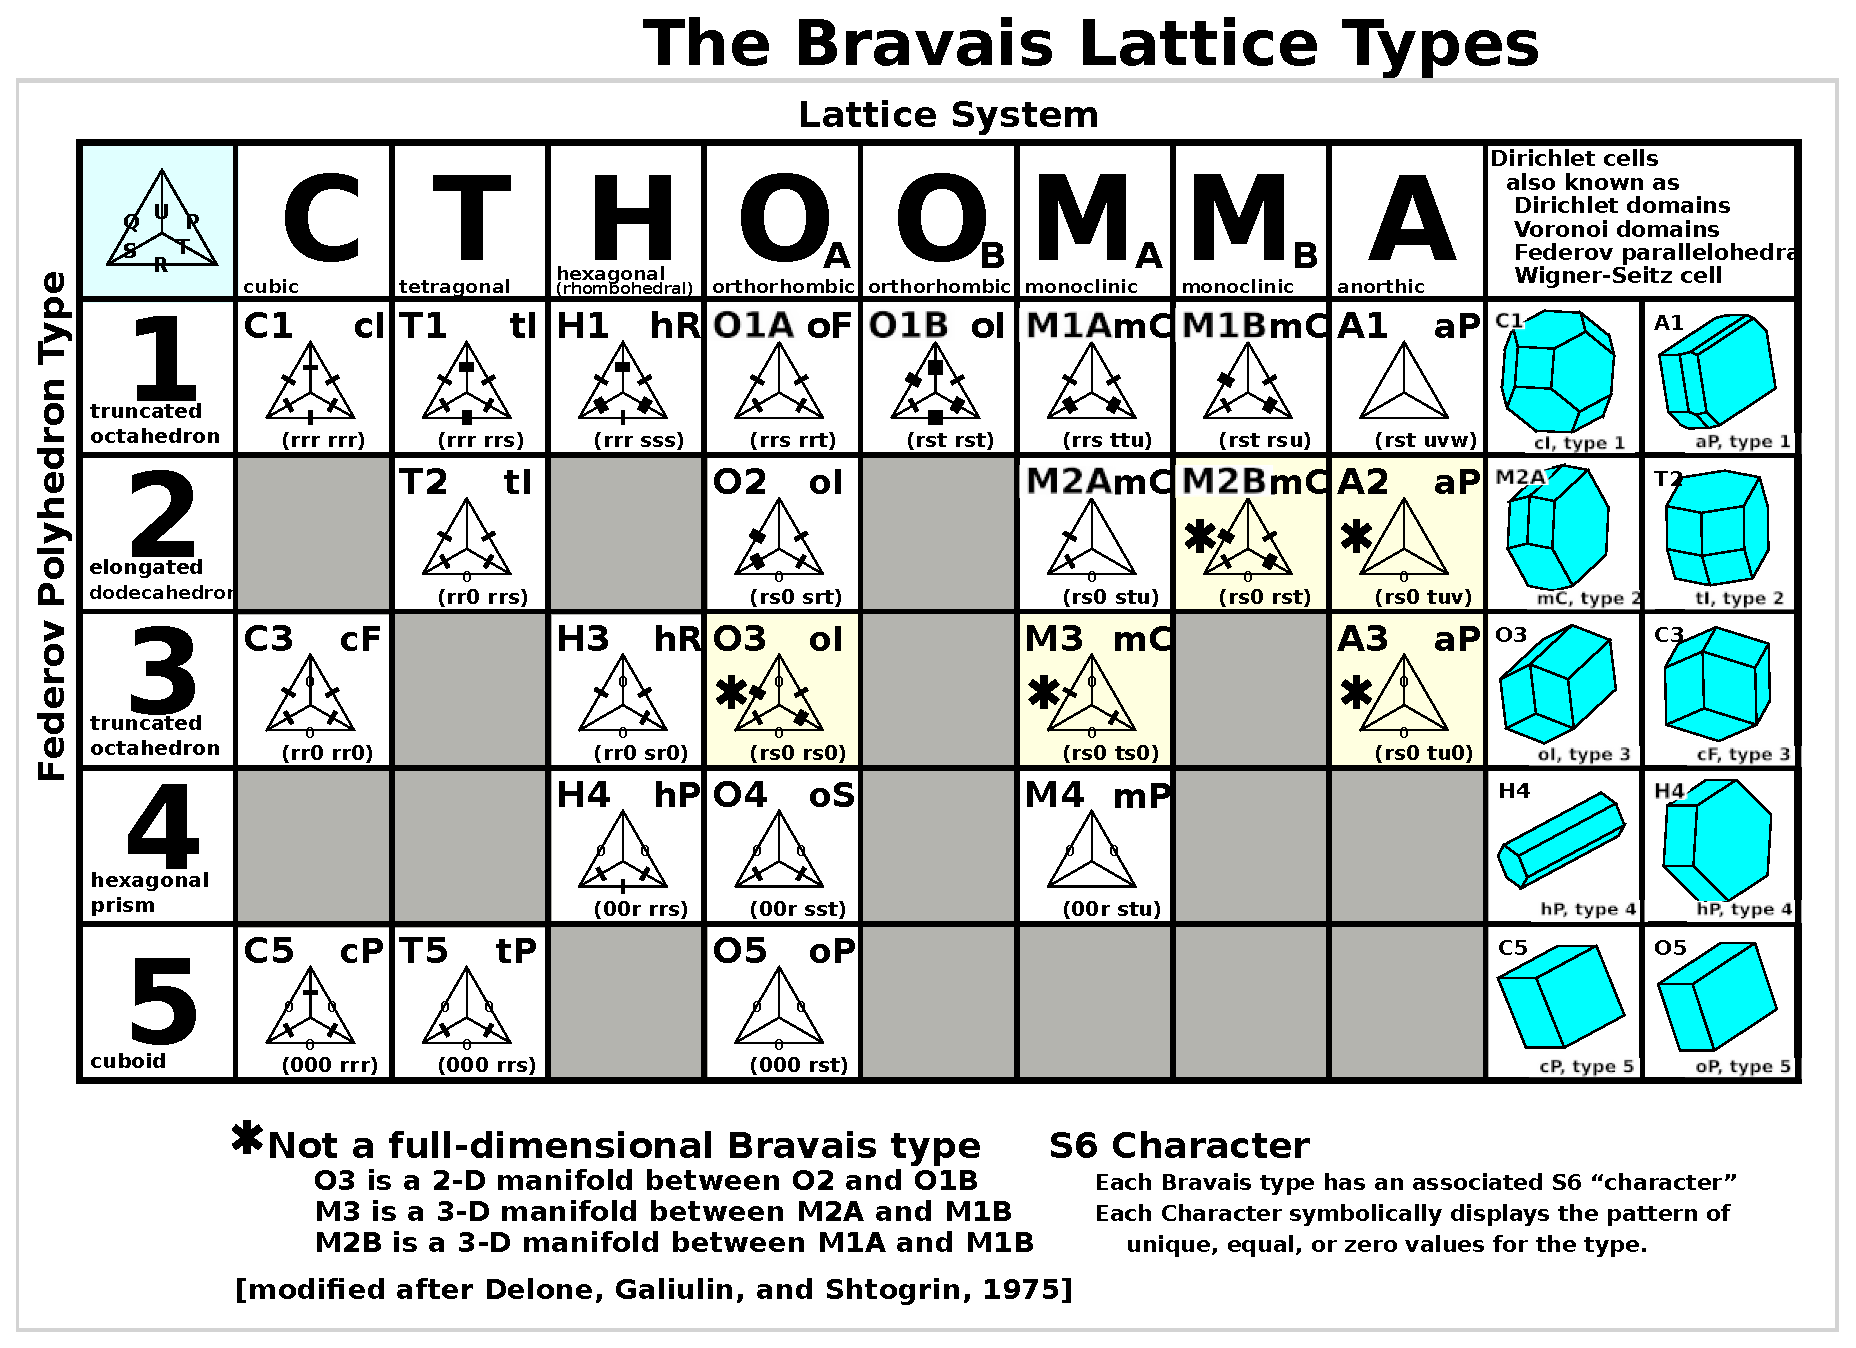
\includegraphics[angle=90, width=0.7\textheight]{DeloneGridClaude_2-3}
		\caption{The Delone types}
		\label{fig:rotatedDeloneTypes}
	\end{figure}
	
	\begin{figure}
		\caption{The O4 item from the Delone Grid with Delone type description}
		\label{fig:O4_terminology}
		
\includegraphics[width=12cm]{O4_terminology}
	\end{figure}
	
	\begin{figure}
		\caption{}
		\label{fig:degenerate}
		\includegraphics[width=12cm]{NullSpaceDistribution}
	\end{figure}
	
	\begin{figure}
		\label{fig:M4}
		\caption{Delone type M4: there are two zeros. A circle of 100 points with
			radius 0.1 is centered at 0,0. The lattices are reduced and the points are
			plotted at the distance from M4. The red points indicate the original
		circle. The blue points are for the reduced cells.}
		\includegraphics[width=12cm]{M4-100-2-zeros}
	\end{figure}
	
	\begin{figure}
		\caption{Delone type O5: there are three zeros. A sphere 
			is centered at 0,0,0, with radius 0.1. The lattices are 
			reduced, and the point is 
			placed at a distance equal to the distance from type O5. 50,000
			points are plotted.}
		\label{fig:O5}
		\includegraphics[width=12cm]{O5-50K-3-zeros}
	\end{figure}
	
	\begin{figure}
		\caption{Delone type O4 (character \charseq{00r stu}): There are two zeros and one pair.			 
			100,000 points are plotted; for each
			 point, the corresponding lattice was reduced; each point
			is assigned a color (0.01) to blue (0.0075),
			according to its reduced distance from the origin.}
		\label{fig:O4}
		\includegraphics[width=12cm]{O4_Cropped-2-zeros-1-pair}
	\end{figure}
	
		
	\bibliography{Reduced}
	
	\bibliographystyle{iucr}
	
	
\end{document}                    % DO NOT DELETE THIS LINE
%%%%%%%%%%%%%%%%%%%%%%%%%%%%%%%%%%%%%%%%%%%%%%%%%%%%%%%%%%%%%%%%%%%%%%%%%%%%%%
